%%%%%%%%%%%%%%%%%%%%%%%%%%%%%%%%%%%%%%%%%%%%%%%%%%%%%%%%%%%%%%%%%%%%%%
% Overleaf (WriteLaTeX) Example: Molecular Chemistry Presentation
%
% Source: http://www.overleaf.com
%
% In these slides we show how Overleaf can be used with standard 
% chemistry packages to easily create professional presentations.
% 
% Feel free to distribute this example, but please keep the referral
% to overleaf.com
% 
%%%%%%%%%%%%%%%%%%%%%%%%%%%%%%%%%%%%%%%%%%%%%%%%%%%%%%%%%%%%%%%%%%%%%%
% How to use Overleaf: 
%
% You edit the source code here on the left, and the preview on the
% right shows you the result within a few seconds.
%
% Bookmark this page and share the URL with your co-authors. They can
% edit at the same time!
%
% You can upload figures, bibliographies, custom classes and
% styles using the files menu.
%
% If you're new to LaTeX, the wikibook is a great place to start:
% http://en.wikibooks.org/wiki/LaTeX
%
%%%%%%%%%%%%%%%%%%%%%%%%%%%%%%%%%%%%%%%%%%%%%%%%%%%%%%%%%%%%%%%%%%%%%%

\documentclass[xcolor=dvipsnames]{beamer}

\usetheme{Madrid}
\useoutertheme{split} % Alternatively: miniframes, infolines, split
\useinnertheme{circles}

%%%%%%%%%%
% Giorgio Morandi #colors_1
\definecolor{color0}{HTML}{372639}
\definecolor{color1}{HTML}{C2A4C0}
\definecolor{color2}{HTML}{816288}
\definecolor{color3}{HTML}{C6926C}
\definecolor{color4}{HTML}{D5BEA9}
\definecolor{color5}{HTML}{DBCAD3}
%%%%%%%%%%

%%%%%%%%%%
\setbeamercolor{normal text}{bg = color5!25, fg = color0}
%\setbeamercolor{alerted text}{bg = color5, fg = color1}
%\setbeamercolor{example text}{bg = color5, fg = color1!50!color0}

\setbeamercolor{palette primary}{bg = color3, fg = color5!50}
%\setbeamercolor{palette secondary}{bg = color1, fg = color5}
%\setbeamercolor{palette tertiary}{bg = color4, fg = color5}

\setbeamercolor{palette quaternary}{bg = color2!50, fg = color0!75}

\setbeamercolor{structure}{bg = color5!50, fg = color4} % itemize, enumerate, etc

\setbeamercolor{section in toc}{bg = color5!50, fg = color1} % TOC sections

% Override palette coloring with secondary
\setbeamercolor{subsection in head/foot}{bg = color3!50, fg = color2}
% For more themes, color themes and font themes, see:
% http://deic.uab.es/~iblanes/beamer_gallery/index_by_theme.html
%%%%%%%%%%

%%%%%%%%%%
\mode<presentation>
{
  \usetheme{Madrid}       % or try default, Darmstadt, Warsaw, ...
  \usecolortheme{default} % or try albatross, beaver, crane, ...
  \usefonttheme{serif}    % or try default, structurebold, ...
  \setbeamertemplate{navigation symbols}{}
  \setbeamertemplate{caption}[numbered]
} 

\usepackage[english, french]{babel}
\usepackage[utf8x]{inputenc}
\usepackage{chemfig}
\usepackage[version = 3]{mhchem}

% On Overleaf, these lines give you sharper preview images.
% You might want to `comment them out before you export, though.
\usepackage{pgfpages}
\pgfpagesuselayout{resize to}[%
  physical paper width = 8in, physical paper height = 6in]
  
% Here's where the presentation starts, with the info for the title slide
\title[Learning program embeddings]{\textsc{Learning student program embeddings using abstract execution traces}}
\institute{\large{\texttt{Présentateur : Hao ZHANG}}}
\author{Auteurs : Guillaume Cleuziou, Frédéric Flouvat}

\usepackage{datetime}
\newdate{date}{8}{7}{2021}
\date{\displaydate{date}}
%\date{11 novembre 2018}

%\logo{
\includegraphics[height = 20mm]{images/logo.png}}

\setbeamersize{text margin left = 0.25in, text margin right = 0.25in}

\usepackage{ragged2e}
\renewcommand{\raggedright}{\leftskip=0pt \rightskip=0pt plus 0.25in}

\begin{document}

\begin{frame}
	\titlepage
\end{frame}

\section{Introduction}

\begin{frame}
\frametitle{Sommaire}
\tableofcontents[currentsection]
\end{frame}

\subsection{Contexte de recherche}
\begin{frame}
\frametitle{Contexte de recherche}
\begin{itemize}
\item[$\bullet$] Généralement, dans les plateformes d’apprentissage de programmation, les apprenants soumettent leur(s) code(s) et la plateforme renvoie toute erreur de syntaxe ou erreur fonctionnelle. L'exploitation de ces données pourra ouvrir de nouvelles perspectives pour suivre et aider les débutants pour apprendre la programmation.

\item[$\bullet$] Cependant, ces plateformes de formation doivent aller au-delà d'une simple analyse syntaxique du script, et permettre de considérer la sémantique associée. À cette fin, l'intégration de programmes d'apprentissage est récemment apparue comme un domaine de recherche prometteur.

\item[$\bullet$] Inspirés du Text Mining, les programmes informatiques peuvent être traités comme du texte et utilisés pour générer une représentation vectorielle et compressée.
\end{itemize}
\end{frame}


\subsection{Le défi}
\begin{frame}
\frametitle{Le défi - I}
\begin{block}{Au niveau des caractéristiques du code}
\begin{itemize}
\item[$\bullet$] Le code a certaines spécificités qui doivent être intégrées pour avoir des représentations aussi riches. Contrairement aux textes, les codes sont exécutables et de petites modifications peuvent avoir des impacts significatifs sur leurs exécutions.

\item[$\bullet$] Un programme peut également appeler d'autres programmes qui peuvent eux-mêmes appeler d'autres programmes. Le contexte dans lequel une instruction est utilisée est également particulièrement important pour en déduire son rôle.

\item[$\bullet$] Enfin, contrairement aux textes, les arbres syntaxiques des programmes sont généralement plus profonds et composés de sous-structures répétitives (boucles).
\end{itemize}
\end{block}
\end{frame}

\begin{frame}
\frametitle{Le défi - II}
\begin{block}{Au niveau des approches existantes}
\begin{itemize}
\item[$\bullet$] Les méthodes existantes pour la construction de l’intégration de programmes intègrent partiellement ces caractéristiques.

\item[$\bullet$] Les approches existantes se concentrent davantage sur la fonction du programme que sur son style.

\item[$\bullet$] De plus, la plupart de ces approches sont supervisées et construisent des intégrations pour une tâche spécifique.
\end{itemize}
\end{block}
\end{frame}

\section{LA MÉTHODE $code2aes2vec$}
\begin{frame}
\frametitle{Sommaire}
\tableofcontents[currentsection]
\end{frame}

\subsection{Deux étapes}
\begin{frame}[fragile]
\frametitle{Deux étapes - I}
\begin{figure}[ht]
\begin{center}
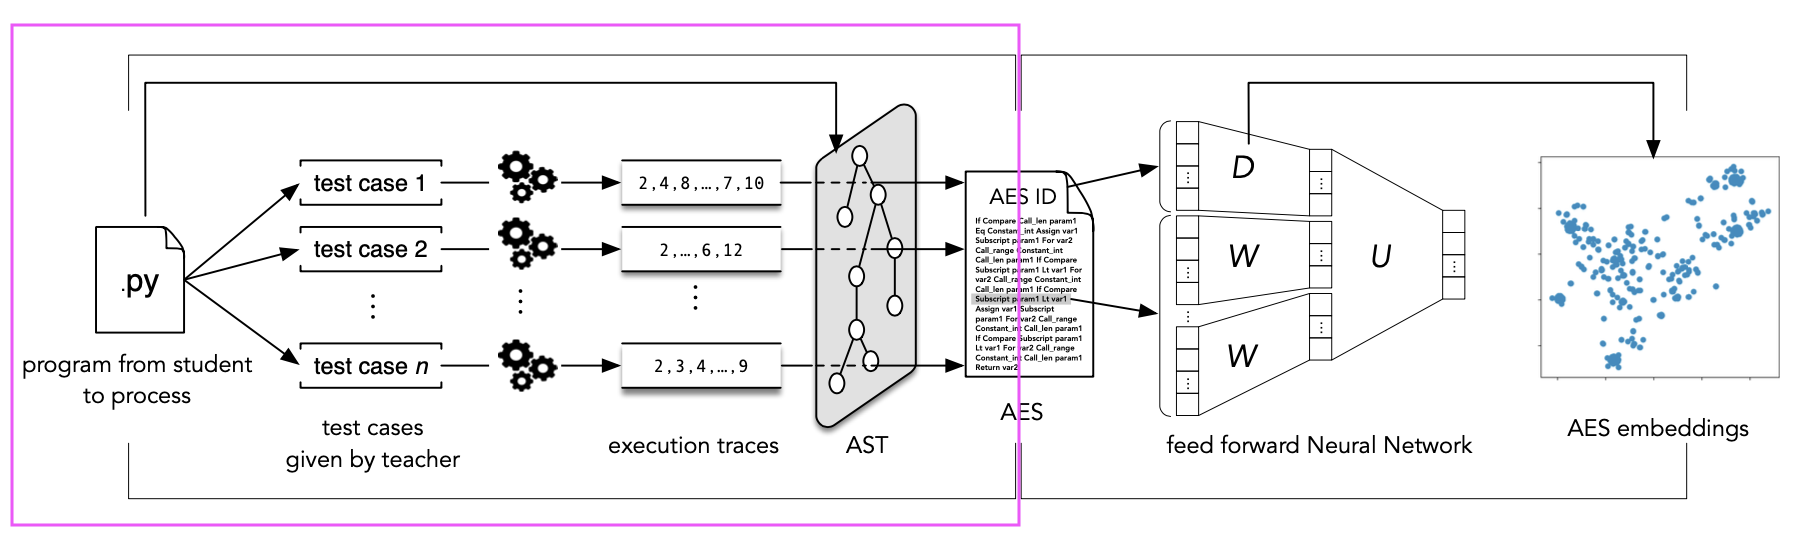
\includegraphics[width=\textwidth]{./images/Figure_1.png}
\vspace{-0.5cm}

\begin{block}{Étape $code2aes$}
Cette étape représente un programme sous la forme d'une séquence d'exécution abstraite (AES), correspondant aux chemins d'arbres de syntaxe abstraite (AST) utilisés par le programme lors de son exécution sur des cas de test prédéfinis.
\end{block}
\end{center}
\end{figure}
\end{frame}

\begin{frame}[fragile]
\frametitle{Deux étapes - II}
\begin{figure}[ht]
\begin{center}
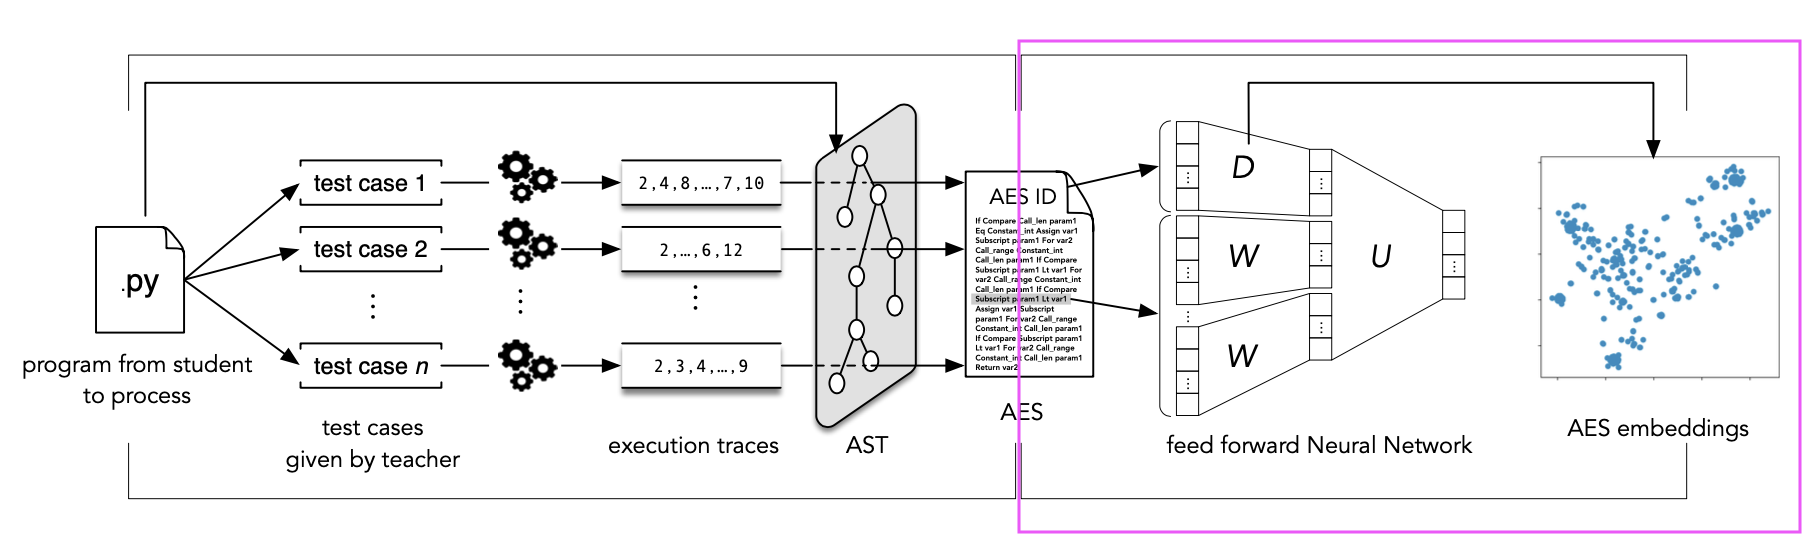
\includegraphics[width=\textwidth]{./images/Figure_2.png}
\vspace{-0.5cm}

\begin{block}{Étape $aes2vec$} 
Cette étape utilise un réseau de neurones pour construire de l’intégration de programmes en fonction de leur AES (en utilisant l'approche $doc2vec$).
\end{block}
\end{center}
\end{figure}
\end{frame}

\subsection{$code2aes$ : construction de séquences d'exécution abstraites (AES)}
\begin{frame}
\frametitle{$code2aes$ : construction de séquences d'exécution abstraites (AES) - I}
Trois niveaux de traduction (ou d'abstraction) sont proposés selon la profondeur considérée dans l'AST :
\begin{itemize}
\item[$\bullet$] AES niveau 0 : chaque ligne de programme est représentée par un mot unique correspondant au symbole de tête du sous-arbre associé dans l'AST (en rouge sur la figure)

\item[$\bullet$] AES niveau 1 : chaque ligne de programme est représentée par un ou plusieurs mots correspondant aux symboles de tête du sous-arbre associé et de ses sous-arbres principaux (en rouge et bleu sur la figure),

\item[$\bullet$] AES niveau 2 : chaque ligne de programme est traduite en une séquence de mots correspondant à tous les nœuds apparaissant dans le sous-arbre associé (en rouge, bleu et noir sur la figure).
\end{itemize}
\end{frame}

\begin{frame}[fragile]
\frametitle{$code2aes$ : construction de séquences d'exécution abstraites (AES) - II}
\begin{figure}[ht]
\begin{center}
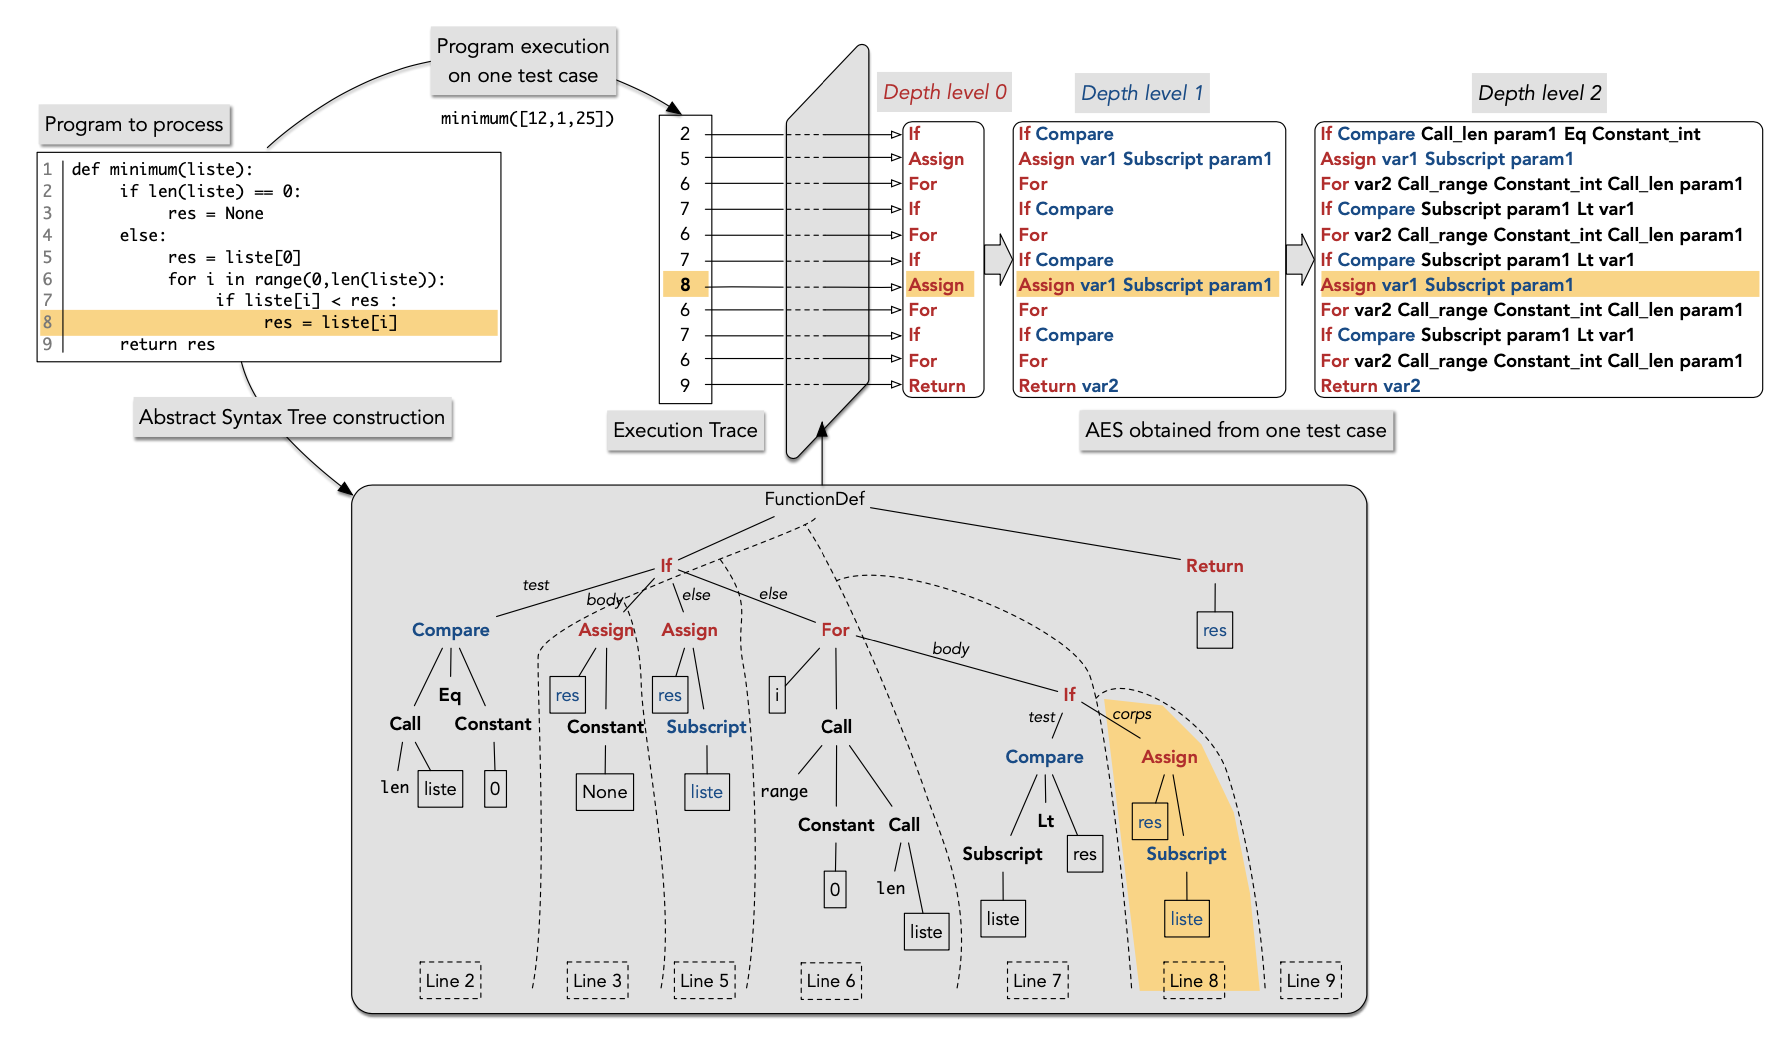
\includegraphics[width= 0.9\textwidth]{./images/Figure_3.png}
\end{center}
\end{figure}
\end{frame}

\subsection{$aes2vec$ : apprentissage des intégrations de programmes d'AES}
\begin{frame}{$aes2vec$ : apprentissage des intégrations de programmes d'AES - I}
\small{
\begin{itemize}
\item[$\bullet$] Les programmes sont considérés comme des documents textuels dont la séquence de mots est donnée par un AES obtenu à l'étape précédente ($code2aes$).

\item[$\bullet$] Dans ce modèle d'apprentissage, chaque vecteur AES est utilisé uniquement pour les prédictions des tokens de cet AES, tandis que les vecteurs de tokens (en $W$ ) sont communs à tous les AES. 

\item[$\bullet$] Une fois le modèle entraîné, la matrice $D$ contient les intégrations des programmes. Les autres paramètres du modèle restant fixes (W ainsi que les paramètres softmax).

\item[$\bullet$] Enfin, le choix de la stratégie d'agrégation utilisée dans la couche cachée peut être déterminant, alors qu'une stratégie de concaténation offre l'opportunité d'exploiter l'ordre des mots au sein du contexte.
\end{itemize}
}
\end{frame}

\begin{frame}{$aes2vec$ : apprentissage des intégrations de programmes d'AES - II}
\begin{figure}[ht]
\begin{center}
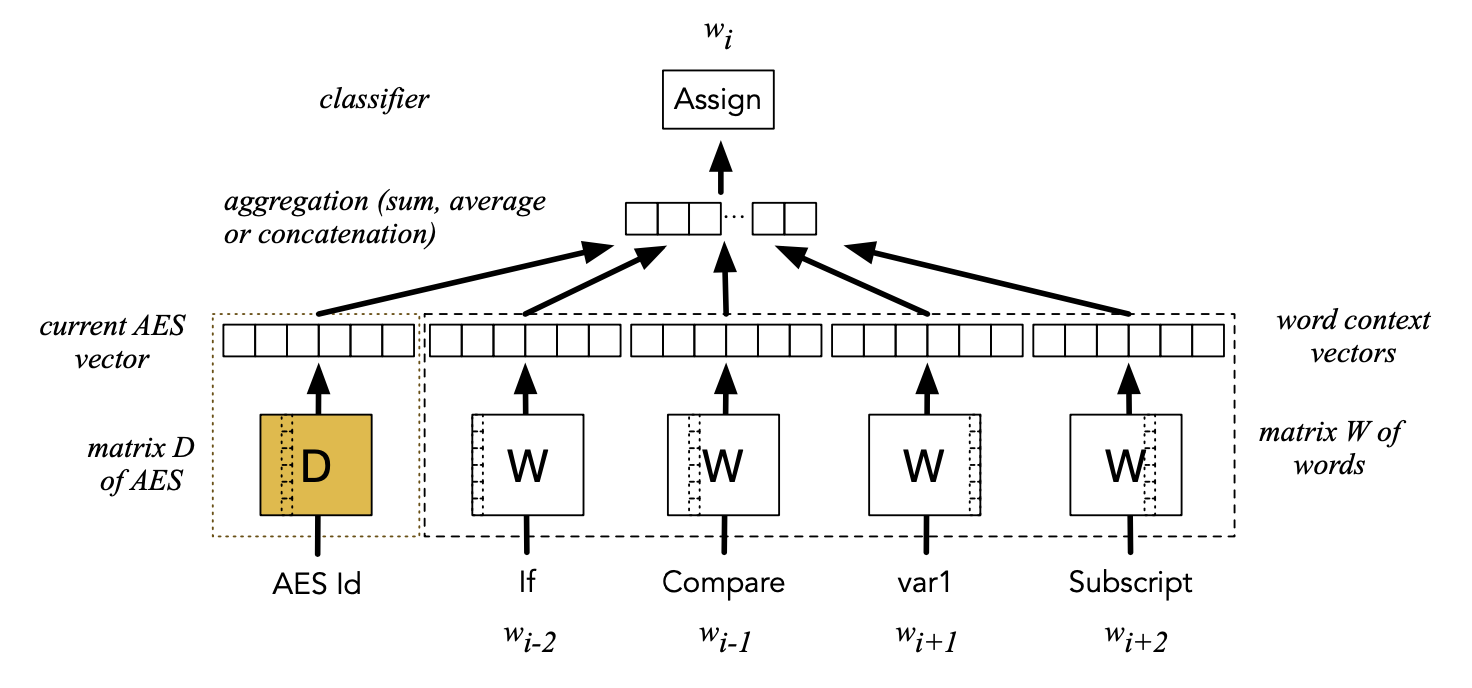
\includegraphics[width= \textwidth]{./images/Figure_4.png}
\end{center}
\end{figure}
\end{frame}

\section{Évaluation de la démarche}

\begin{frame}
\frametitle{Sommaire}
\tableofcontents[currentsection]
\end{frame}

\subsection{Évaluation de manière qualitative}
\begin{frame}[fragile]
\begin{center}
\frametitle{Évaluation de manière qualitative}
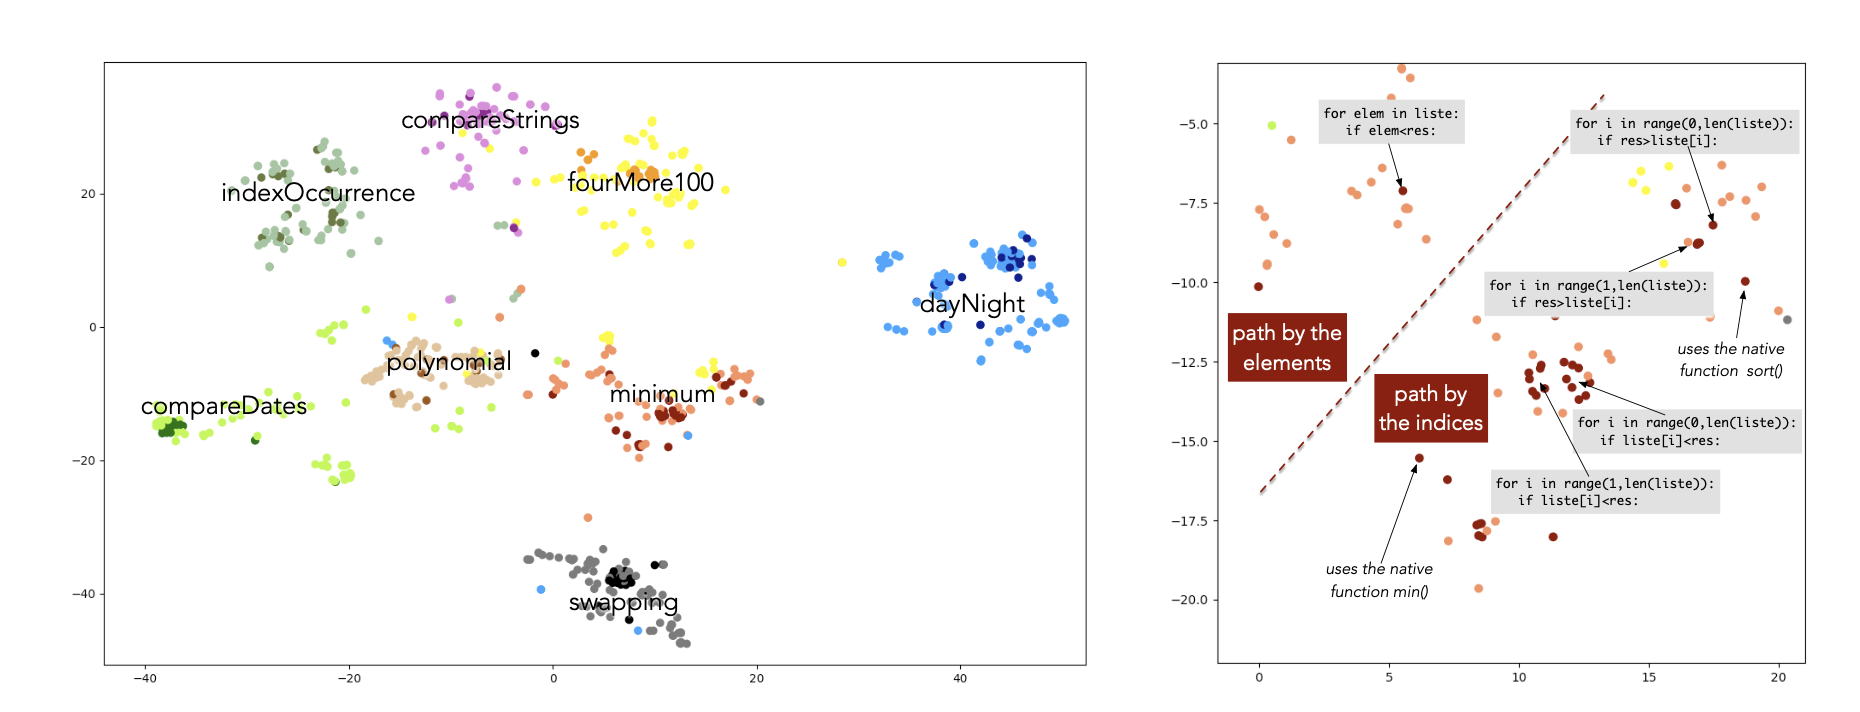
\includegraphics[width= \textwidth]{images/Figure_5.png}
\end{center}

\begin{itemize}
\item[$\bullet$] Stylistique

\item[$\bullet$] Ordre des mots

\item[$\bullet$] Quelques programmes valables, mais atypiques
\end{itemize}

\end{frame}


\subsection{Évaluation de manière quantitative}
\begin{frame}[fragile]
\begin{center}
\frametitle{Évaluation de manière quantitative}
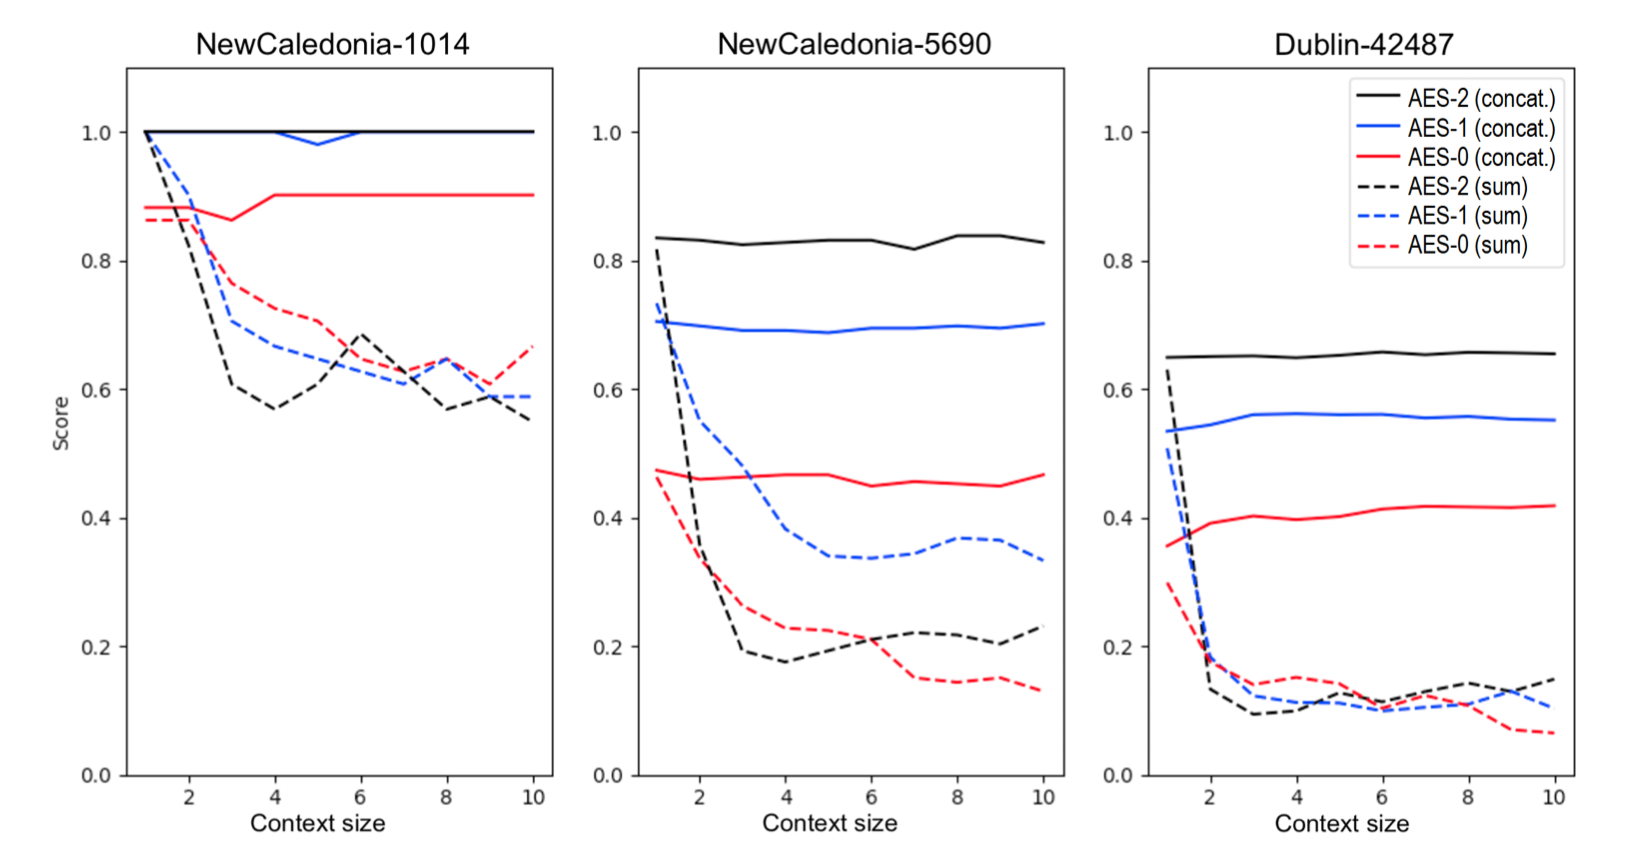
\includegraphics[width= \textwidth]{images/Figure_6.png}
\end{center}
\end{frame}


\subsection{Application à la propagation du feed-back}
\begin{frame}[fragile]
\begin{center}
\frametitle{Application à la propagation du feed-back}
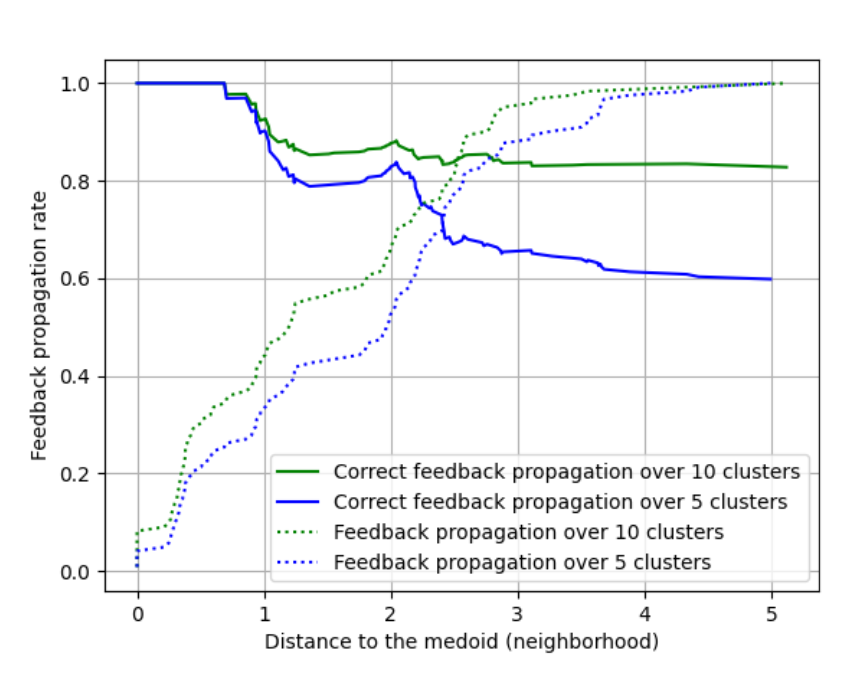
\includegraphics[width= 0.5\textwidth]{images/Figure_7.png}
\vspace{-0.5cm}
\end{center}
La figure montre l'évolution du taux de rétroaction correct en fonction de la taille du voisinage considéré pour la propagation. On peut voir que plus on s'éloigne des médoïdes, plus il y a d'erreurs dans les rétroactions déterminées automatiquement.
\end{frame}


\section{Perspectives d'avenir}
\begin{frame}[fragile]
\frametitle{Perspectives d'avenir}
\begin{itemize}
\item[$\bullet$] Analyser des phrases plus complexes

\item[$\bullet$] Autres langages de programmation
\end{itemize}

\end{frame}

\end{document}